%\section{Materiales y métodos}
\section{Modelos de simulación de la ecología del vector}
La distribución geográfica de larvitrampas, como puntos de control, permite generar información
regionalizada sobre el estado de las poblaciones del vector \cite{NINO2011}, en donde esta
información puede ser combinada con información ambiental, demográfica o epidemiológica, con el
fin de obtener modelos detallados que tengan la capacidad de monitorear, simular el comportamiento
del vector y en consecuencia, predecir una posible epidemia del dengue.

\subsection{Modelo matemático del ciclo de vida}
El modelo considera un espacio bi-dimensional, con un sistema de coordenadas geográficas $(x,y)$,
para expresar todas las posiciones sobre el plano, correspondientes a la longitud y latitud. Si
consideramos a $m_{i}$ como a un individuo que se encuentra en una etapa del ciclo de vida del
Aedes aegypti, correspondiente a una población de mosquitos, entonces, $m_{i}(x,y)$ representa a
$m_{i}$ en las coordenadas geográficas $(x,y)$.

Se consideran seis poblaciones diferentes: los huevos $H(x,y)$, larvas $L(x,y)$, pupas $P(x,y)$,
machos adultos $AM(x,y)$, hembras adultas nulíparas\footnote{Hembras que no han ovipuesto.}
$AN(x,y)$ y hembras adultas paridas\footnote{Hembras que han ovipuesto al menos una vez.} $AP(x,y)$. En algunos procesos se utiliza $A(x, y)$ para representar a toda la población de adultos,
$AM(x,y)$, $AN(x,y)$ y $AP(x,y)$ correspondientes a $(x, y)$. El modelo considera que todas las
poblaciones cuentan con una cantidad entera de individuos.

La evolución de las poblaciones, se ven afectadas por los siguientes eventos: muerte de huevos,
eclosión de huevos, muerte de larvas, emergencia de pupas, muerte de pupas, emergencia de adultos,
muerte de adultos, ovipostura de hembras nulíparas, ovipostura de hembras paridas y dispersión
de los adultos (machos y hembras). Según \cite{otero2006stochastic}, los eventos se producen a
tasas que dependen no sólo de valores de la población, sino también de la temperatura, que a su
vez es una función de tiempo, por lo tanto, la dependencia de la temperatura introduce una
dependencia del tiempo en las tasas de eventos.


\subsection{Zonificación}
\label{subsec:cap4-zonificacion}
Cada entorno puede contar con factores que lo hagan más o menos apto para el desarrollo,
mortalidad, alimentación, disperción, y reproducción de individuos. En esta sección, con el fin de
simplificar ciertos aspectos muy especificos que se encuentran fuera del alcance de este trabajo,
realizaremos ciertas hipótesis generales, justificadas para nuestro caso de aplicación, pero puede
requerir una revisión en el caso general. Estas hipotesis son, los valores observados en un
conjuto de puntos de control, pertenecientes a una zona, permiten la caracterización de dicha zona como más o menos apta para desarrollo, mortalidad, alimentación, disperción, y reproducción de
individuos. Tambien consideramos que el tamaño de la zona, y por ende la cantidad de puntos de
control que pertenecena ella, influye en la caracterización de las zonas.

La zonificación surge ante necesidad de dividir el espacio de estudio de una forma más granular,
para identificar a los individuos que pertenecen a zonas aptas y los que no. Los puntos de control
distribuidos en un área de estudio nos permite estimar cuales zonas los niveles de riesgo e
infestación correspondiente a la abundacia de larvas por litro que se pueden observar.

En la \tabref{tab:cap4-puntaje-zona} se puden observar los rangos definidos para cada tipo de
zona, en donde $u(x,y)$ es la densidad relativa en un radio, $r$ , donde el valor de la densidad
realtiva es calculado mediante la ecuación \eqref{eq:interpolacion-idw}. Las límites para las
zonas fueron determinados clasificando los valores, de las hembras reproductivas en, grupos
múltiplos de cinco. No se estableció  un límite superior para las zonas óptimas debido a que los
valores mayores a el mínimo establecido, 70 larvas por litro, pertenecen a la misma categoría.

El tamaño del radio,$r$, es un parametro ajustable del modelo, mientras más grande sea el tamaño
del radio, más puntos serán incluidos para el cálculo, lo que gerará que las zonas tiendan a ser
similares.
Para el calculo de las hembras adultas y reproductivas para la clasificación de las zonas se
tuvieron en cuenta los siguientes criterios:

\begin{itemize}
    \item Solo el 50 \% de las larvas observadas son hembras.
    \item La temperatura media utilizada es de 25 \textcelsius.
    \item La mortalidad díaria natural bajo optimas condiciones,a 25 \textcelsius, es de 0,01
    según \eqref{eq:mortalidad-natural-larvas}.
    \item La tasa de desarrollo, a 25 \textcelsius, de la larva hasta su emergencia a adulto es de
    $11.57$ días \citep{rueda1990temperature}.
    \item El 32,10 \% de las hembras adultas no ovipone \citep{osoriopontificia}.
\end{itemize}


\begin{table}
    \begin{minipage}{\textwidth}
\begin{center}
    \caption{\label{tab:cap4-puntaje-zona} Clasificación de las zonas de acuerdo a la densidad de larvas por litro.}
    \begin{tabular}{p{3cm} c c c c}
        \\
                     & Mínimo$^a$ & Máximo$^a$ & Hembras     & Hembras$^c$ \\
        Tipo de zona & $u(x,y)$   & $u(x,y)$   & Adultas$^b$ & Reproductivas$^c$ \\
        \hline
        \hline\\
        Pésima  & 0  & 19 & 8  & 5 \\
        Mala    & 20 & 35 & 15 & 10\\
        Regular & 36 & 51 & 22 & 15\\
        Buena   & 52 & 69 & 30 & 20\\
        Óptima  & 70 & --$^d$ & --$^d$ & --$^d$\\
    \end{tabular}
    \footnotetext[1]{Rango mínimo y máximo de $u(x,y)$ permitido para el tipo de zona.}
    \footnotetext[2]{Cantidad máxima de hembras adultas, al final del periodo de desarrollo.}
    \footnotetext[3]{Cantidad de hembras adultas con capacidad de oviponer.}
    \footnotetext[4]{No se estableció un límite superior para las zonas óptimas. }
\end{center}
    \end{minipage}
\end{table}

\subsection{Tasas de desarrollo}
Se consideran 5 tasas de desarrollo correspondiente a : la eclosión de huevos,
emergencia a pupas, emergencia a adultos, el ciclo gonotrófico de hembras nulíperas y el ciclo gonotrófico de hembras paridas. Las tasas de desarrollo son calculadas mediante la versión simplificada del modelo de Sharpe y DeMichele, presentado en \cite{sharpe1977reaction},
con inhibición de altas temperaturas de Schoolfield.

\begin{equation} \label{eq:schoolfield}
   R(k)  = R(298K) *\cfrac{ \cfrac{k}{298K} *
    exp \Bigg[
            \cfrac{\Delta H_{A}}{R} \bigg(\cfrac{1}{298K} - \cfrac{1}{k}\bigg)
        \Bigg]}
    {1 + exp\Bigg[\cfrac{\Delta H_{H}}{R} \bigg(\cfrac{1}{T_{1/2}}- \cfrac{1}{k}\bigg)\Bigg] }
\end{equation}

Donde $R(k)$ representa la tasa de desarrollo media ($dias^{-1}$) para una temperatura $K$,en la
escala de Kelvin; $T_{1/2}$ es la temperatura cuando la mitad de la enzima se desactiva, debido a
la alta temperatura, mientras que $\Delta H_{A}$ y $\Delta H_{H}$  son entalpías termodinámicas características del organismo, y $R$ es la constante universal de los gases, igual a
$1,987202$ $cal/K.mol$. Los parámetros $R(298K)$, $\Delta H_{A}$, $T_{1/2}$, y $\Delta H_{H}$ son estimados mediante la de regresión no lineal de Wagner, presentado en \cite{wagner1984modeling}.
Según \cite{otero2006stochastic}, el modelo simplificado de Schoolfield, es lo suficientemente
flexible para el ajuste de los datos biológicos disponibles. Los parámetros deben calcularse para
cada etapa de desarrollo, una vez determinados, la ecuación puede utilizarse para calcular tasas
de desarrollo a cualquier temperatura \cite{rueda1990temperature}.


\subsection{Mortalidad}
\label{subsec:cap4-mortalidad}
La mortalidad de los individuos depende de la etapa del ciclo de desarrollo en el que se encuentren
los individuos de una población.

El modelo considera que todas las poblaciones cuentan con una cantidad entera de individuos, por
lo que a la hora de reducir una población se espera que sea mediante la sustracción de una
cantidad entera.La utilización de las tasas de desarrollo dan como resultado cantidades no enteras, por lo que es necesario un pequeño ajuste dado por el siguiente operador de redondeo :

\begin{equation}
\label{eq:operador-redondeo}
\rho(n) = \left\{
\begin{array}{l l}
   round(n) & \quad  \forall n < round(n)\\
   n & \quad  \forall n > round(n)\\
\end{array} \right.
\end{equation}

Donde $round(n)$ es la función redondea, $n$, al entero más cercano. Para $n > round(n)$, la parte
no entera de $n$ queda acumulada para la siguiente iteración.

\subsubsection{Mortalidad de huevos}
La tasa de mortalidad de los huevos se encuentra definida como una constante, $me = 0.01$,
$1/\text{días}$, independiente de la temperatura\citep{otero2006stochastic}.

\begin{equation}
    M_{H(x,y)} = \rho(me * H(x,y))
\end{equation}

Donde $M_{H(x,y)}$ es la cantidad de huevos que deben ser eliminados de la población $H(x,y)$.

\subsubsection{Mortalidad de larvas}
En \citet{otero2006stochastic} la mortalidad de las larvas, se encuentra dividida en dos
contribuciones. La primera contribución representa la mortalidad natural bajo óptimas condiciones
y se encuentra influneciada únicamente de la temperatura. Esta tasa se encuentra definida por :

\begin{equation}
 \begin{array}{l l}
    ml(k) = 0.01 + 0.9725 * exp\bigg( \frac{-(k - 278)}{2.7035}\bigg) &\quad  \forall k, 278 K \geq k \geq 303 K\\
\end{array}
\end{equation}

La segunda contribución es la mortadiad denso dependiente de las larvas. Este mecanismo de
regulación puede estar realacionado con procesos concurrentes, como las limitaciones de los
alimentos, las interacciones químicas, presencia de depredadores especializados en el sitio de
reproducción y mucho más\citep{otero2006stochastic}. Esta se encuentra definida por :

\begin{equation}
  \alpha (x,y) = \alpha _{0}/BS(x,y)
\end{equation}

Donde $\alpha _{0}$ está asociado a la capacidad de carga de un solo lugar de reproducción y
$BS(x,y)$ es el número de sitios de reproducción. El valor de $alpha _{0}$ puede ser instalado en
los valores observados en la región que se está simulando.

Tomando ambas contribuciones, la mortalidad natural bajo óptimas condiciones y la denso
dependiente, la mortalidad de las larvas queda definida como :
\begin{equation}
    M_{L(x,y)}(k) = \rho(ml(k) * L(x,y) + \alpha (x,y) * L(x,y) *(L(x,y) - 1))
\end{equation}

Donde $M_{L(x,y)}$ es la cantidad de larvas que deben ser eliminadas de la población $L(x,y)$.

\subsubsection{Mortalidad de las pupas}
La tasa de mortalidad de las pupas se encuentra definida como una función influneciada únicamente
de la temperatura. \citep{otero2006stochastic}.

\begin{equation}
 \begin{array}{l l}
    mp(k) = 0.01 + 0.9725 * exp\bigg( \frac{-(k - 278)}{2.7035}\bigg) &\quad  \forall k, 278 K \geq k \geq 303 K\\
\end{array}
\end{equation}

Además de la mortalidad diaria en la fase de pupa, existe una importante mortalidad adicional
asociada con la emergencia sin éxito de adultos, solo el 83\%  de las pupas alcanzan la maduración
y emergerán como mosquitos adultos, por lo tanto, el factor de supervivencia es de $ef=0.83$
\citep{otero2006stochastic}.

\begin{equation}
    M_{P(x,y)}(k) = \rho(P(x,y) * (mp + (1 - ef) * R(k)))
\end{equation}

Donde $M_{P(x,y)}$ es la cantidad de pupas que deben ser eliminadas de la población $P(x,y)$.

\subsubsection{Mortalidad de adultos}
La tasa de mortalidad de los adultos se encuentra definida como una constante, $ma = 0.09$,
$1/\text{días}$, independiente de la temperatura\citep{otero2006stochastic}.

\begin{equation}
    M_{A(x,y)} = \rho(ma * A(x,y))
\end{equation}

Donde $M_{A(x,y)}$ es la cantidad de adultos que deben ser eliminados de la población $A(x,y)$.

\subsection{Sitios de reproducción}
\label{subsec:cap4-sitios de reproduccion}
Sea $BS$ el número de sitios de reproducción agrupados como uno solo para una determinada zona. La
variable ambiental, $BS$ ,determina el tamaño de la población de equilibrio en el modelo
determinista \cite{otero2006stochastic, otero2008stochastic}. Las diferentes condiciones
ambientales deben ser representadas por diferentes valores del parámetro de $BS$
\cite{otero2008stochastic}.

Se considera a $BS(x,y)$ como el valor de $BS$, asociado a $(x,y)$, partiendo de las hipótesis
realizadas en la \secref{subsec:cap4-zonificacion} podemos considerar que el valor de $BS(x,y)$ se
encuentra influenciado por $u(x,y)$, de ese modo a medida que $u(x,y)$ varíe, lo debe hacer el
valor de $BS(x,y)$. Para el cálculo de $BS$ relativo a $(x,y)$ se utiliza el método interpolador
de Lagrange.

Sea $bs$ la función a interpolar, sean $u_0$, $u_1$,...,$u_m$ las densidades conocidas de $bs$ y
sean $bs_0$, $bs_1$,...,$bs_m$ los valores que toma la función para dichas densidades, el polinomio interpolador de grado n de Lagrange es un polinomio de la forma :

\begin{equation}
\label{eq:sitios-reproduccion-x-y}
    bs(u(x,y)) = \sum_{i=0}^{n} bs_{i} * l_{i}(u(x,y))
\end{equation}

donde $l_j(u(x,y))$ son los llamados polinomios de Lagrange, que se calculan de este modo:

\begin{equation}
\label{eq:sitios-reproduccion-x-y}
    l_{i}(u(x,y)) = \prod_{j \neq i} \cfrac{u(x,y) - u_{j}}{u_{i} - u_{j}}
\end{equation}

Consideramos un polinomio de tercer grado, con los parámetros $u_0$, $u_1$ y $u_2$ igual a $19$,
$51$ y $70$, correspondientes a zonas del tipo \textit{Pésima}, \textit{Regular} y \textit{Óptima}.
Los valores, $bs_{min}$, $bs_{med}$ y $bs_{max}$ respectivamente, estos son parámetros
configurables del modelo donde $bs_{min}$ representa el menor $BS$ observado, $bs_{max}$
representa el mayor $BS$ observado y  $bs_{med}$ es el valor medio existente entre $bs_{max}$ y
$bs_{min}$.

\subsection{Ciclo gonotrófico y Ovipostura}
\label{subsec:cap4-ciclo-gontrofico-ovipostura}
El Aedes aegypti puede alimentarse más de una vez para cada ovoposición \cite{scott1993detection},
especialmente si es perturbado antes de finalizar si alimentación. En \cite{osoriopontificia},
observa que  22.56 \% de la población no realizó ninguna toma de sangre, por ende no generó
ninguna tanda de huevos,  43.6 \% realizaron una toma de sangre, de las cuales el 21.9\% de los
mosquitos no realizaron ovoposturas, 16.5 \% realizaron dos tomas de sangre, 8.42 \% realizaron
tres tomas de sangre, 6.9 \% realizaron cuatro tomas de sangre y 2.02 \% realizaron cinco tomas de
sangre. La cantidad de huevos en cada oviposición, luego de las alimentaciones sanguineas
correspondientes, varía entre 30 y 100 unidades \cite{luevano1993ciclo, beltran2001bionomia,cabezas2005dengue}.

El ciclo gonotrófico de los mosquitos es el nombre que se le adjudico al período que existe desde
que el mosquito realiza una alimentación sangínea - ovipostura - hasta una nueva alimentación.
Como se mencionó anteriormente en \secref{subsec:cap4-tasas de desarrollo}, la tasa de desarrollo
del ciclo gonotrófico puede estimarse mediante la versión simplificada del modelo de Sharpe y DeMichele \cite{sharpe1977reaction}, popuesta por Schoolfield en \cite{schoolfield1981non}.

Sea $R(k_{i})$ la tasa de desarrollo (ver ecuación \eqref{eq:schoolfield}) del ciclo gonotrófico
de una hembra (nulípara, parida), para una temperatura de $k_{i}$ Kelvin en un instante $i$, se
considera que un día es de ovipostura si se cumple :

\begin{equation}
\label{eq:ciclo-gonotrofico-ovipostura}
    \sum_{i=0}^{N} R(k_{i}) \geq 1
\end{equation}

Donde $N$ es la duración en días del ciclo gonotrófico de la hembra. Para $R(k)$ se aplican los
parámetros correspondientes a hembras nulíparas y paridas de acuerdo al estado de la hembra.
En \cite{edman1987host} se observó que hembras nulíparas de Aedes aegypti poseen un proceso de
digestión es más lento en las hembras paridas y por ende el ciclo gonotrófico de las mismas tiene
a ser más largo.


\subsection{Vuelo y dispersión}
\label{sec:cap4-vuelo-dispersion}
El aedes aegypti es un mosquito doméstico que generalmente esta confinado a las casas donde se
cria \citep{luevano1993ciclo}, tiende a permanecer físicamente en donde emergió, siempre y cuando
no exista algún factor que la perturbe o no disponga de huéspedes, sitios de reposo y de postura
\citep{ThironIzcazaJ2003}. Por lo general mosquito no sobrepasa los 50 a 100 metros durante su vida
\citep{cabezas2005dengue}. En caso de no contar con sitios adecuados de ovipostura y disponibilidad
de alimento tienden a dispersarme una mayor distancia, hasta tres kilómetros, en busca de
mejores condiciones \citep{ThironIzcazaJ2003}. Los mosquito tienen la particularidad de que vuelan
en sentido contrario al la dirección al viento \citep{ThironIzcazaJ2003} y a una velocidad máxima
de $2 km/h$\citep{kaufmann2004flight}.

Exiten varios factores externos, que influyen el la dispersión del mosquito, disponiblidad de
alimentos, criadreos, sitios de reposo. Para las estrategias de control de Aedes aegypti en zonas
urbanas donde existen brotes de dengue y fiebre amarilla se asume que los mosquitos tienen un
rango de vuelo durante su vida de 50 a 100 metros\citep{dengueUruguayCap8}.

La función más importante del adulto de Aedes aegypti es la reproducción y secundariamente la
dispersión de la especie. Para Aedes aegypti el transporte pasivo de huevos y larvas en
recipientes ha tenido mayor trascendencia en su distribución, en la que el hombre ha participado
en forma determinante en comparación con la dispersión activa propia de la especie
\citep{ThironIzcazaJ2003}.

Para la dipsersión de los mosquitos consideramos a la zonificación como una aproximación válida
para la caracterización del habitad del mosquito. Para zonas de riegos calificadas como Malas o
Pésimas el rango de vuelo del mosquito se encuetra definido entre 100 metros a 3 kilometros y para
las demás zonas que no cumplan con dicho criterio el rango de vuelo se encuentra entre 0 y 100
metros. De este modo, los mosquitos que se encuentren en zonas menos aptas tenderán a desplzarce
en busca de mejores condiciones.


\section{Simulación del proceso evolutivo}
La simulación del proceso evolutivo es el encargado de simular los efectos de las variaciones
climáticas y el entorno en el ciclo de vida del Aedes aegypti.

El simulador del proceso evolutivo, es considerado como un proceso iterativo que inicia tomando
como parámetros de entrada la población inicial, y los datos climatológicos correspondientes al
periodo de simulación seleccionado. La población inicial es obtenida mediante la cantidad de
larvas observadas en los puntos de control que corresponden a la muestra utilizada para el estudio.
Por cada larva observada, en un punto de control ubicado en las coordenadas geográficas, $(x, y)$,
se inicializa un individuo con las mismas coordenadas del punto de control de origen.

\begin{figure}[!t]
    \centering
    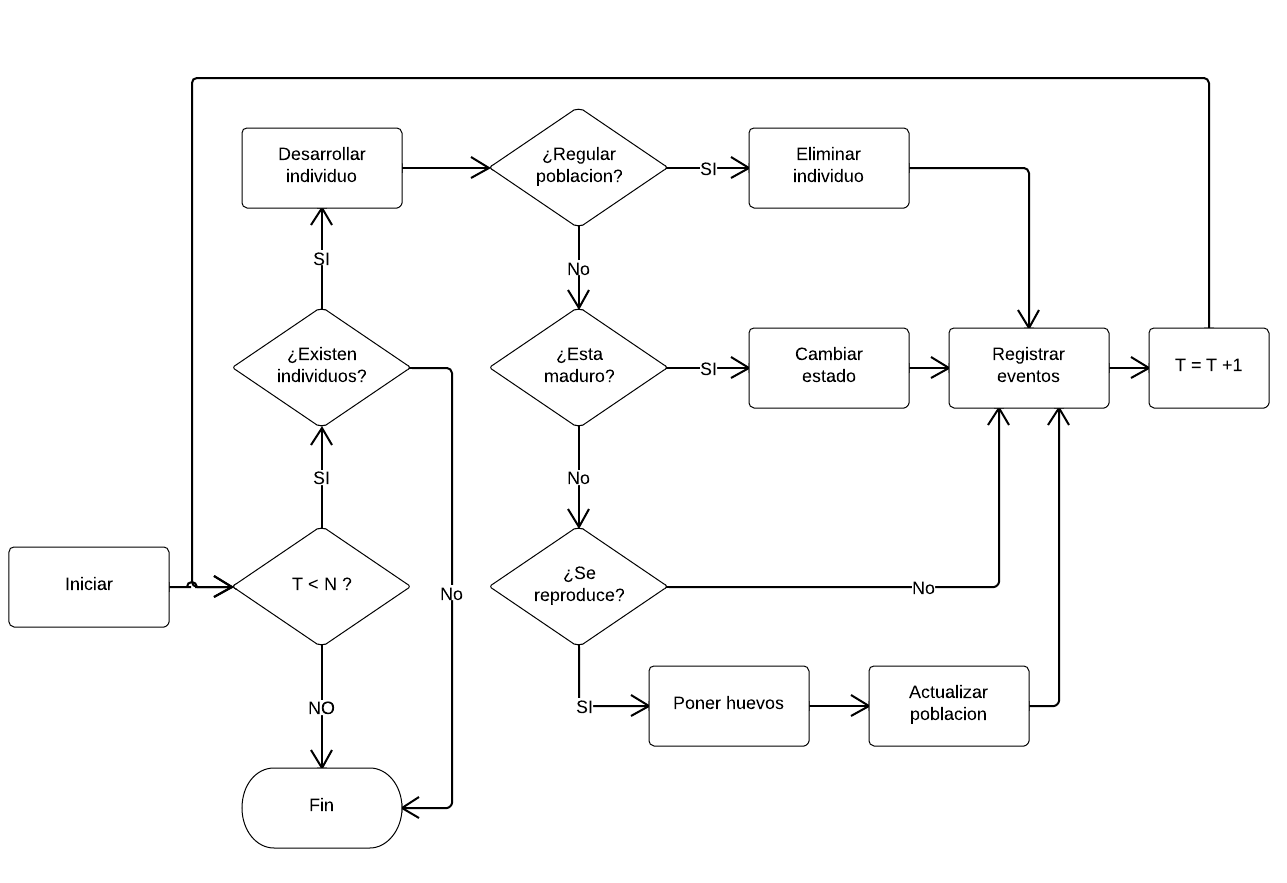
\includegraphics[width=0.45\textwidth]{../book/capitulo-5/graphics/algoritmo-evolutivo.png}
    \caption{\label{fig:algoritmo-evolutivo}Algoritmo del simulador del proceso evolutivo.}
\end{figure}

En la \figref{fig:algoritmo-evolutivo} se presenta el algoritmo del proceso evolutivo, donde el
periodo de simulación se encuentra representado por $T$.  El desarrollo de los individuos se
encarga de calcular las tasas de desarrollo correspondientes para cada etapa de su ciclo de vida,
con el fin de estimar su desarrollo considerando las condiciones climáticas. El cambio de estado
es consecuencia de la finalización de la etapa de desarrollo del individuo, donde el individuo ya
está listo para pasar a la siguiente etapa de su ciclo de desarrollo.

La regulación de la población es la encargada de calcular las tasas de mortalidad diaria,
correspondientes a cada etapa del ciclo de desarrollo del individuo, con el fin de reducir el
tamaño de la población debido a la mortalidad diaria de los individuos.

Si el individuo en cuestión corresponde a una hembra adulta inseminada, entonces esta se encuentra
en fase reproductiva. La postura de huevos se realiza respetando la tasa de desarrollo del ciclo
gonotrófico de las hembras. Si la hembra adulta ovipone, los huevos son añadidos a la población
como individuos en un estado inicial de \textit{HUEVO}.


